\documentclass[UTF8,12pt,a4paper]{ctexart}
\usepackage{amsmath,amssymb,booktabs,geometry,graphicx,float,hyperref}
\geometry{left=2.5cm,right=2.5cm,top=2.5cm,bottom=2.5cm}
\graphicspath{{figs/}{./}}
\newcommand{\keywords}[1]{\par\noindent\textbf{关键词：}#1}
\newcommand{\pos}[1]{\left[#1\right]^+}
\title{微网与外部电网电力调控策略研究（更新稿）}
\author{}
\date{}
\begin{document}
\maketitle

\begin{abstract}
本文研究固定与波动电价、负荷和光伏信息逐步揭示条件下的微网购电与储能调度。以十分钟为离散步长，建立显式区分常规购电、紧急购电、充放电和未利用供能的能量平衡模型，并检查储能功率、状态边界和跨日状态。问题一采用带互斥约束的混合整数线性规划，并以5\,kWh有限状态网格的库存价值动态规划独立交叉核验；问题二采用目标日前同类型日的日电量—日内形状负荷预测和三日光伏中位数的0.9保守校准；问题三在0、6、12、18时锁定已执行前缀并滚动重优化，严格按计划基准费、调减0.5倍、调增1.5倍和紧急费结算；问题四在附件4波动价格下从相同日初储能状态独立计算两个分支。问题一购电量为59482.699\,kWh、费用为35126.986\,元；2025年2月1日至12月31日的本地回测费用分别为Q2 16206550.45\,元、Q3 18242015.85\,元、Q4-2 16989713.48\,元和Q4-3 19577410.54\,元。所有数值均由当前附件和代码生成，不代表官方成绩。
\end{abstract}
\keywords{微网；储能调度；混合整数线性规划；库存价值；滚动调整；动态电价}

\section{问题重述与数据审计}
题面要求在十分钟粒度给出微网的计划购电、紧急购电和储能充放电策略。附件1提供单日固定价格、负荷及光伏预测；附件2提供2025年全年实际负荷和光伏；附件3在每天0、6、12、18时发布未来24小时整点光伏预报；附件4提供全年波动价格。本文把标签0:10至0:00+1解释为对应当天0:00--24:00的区间末，功率乘\(\Delta t=1/6\) h后转为电量。全年回测严格切片为2025-02-01至2025-12-31，共334天；目标日的预测只读取早于该日的历史行。题面与规则以官方材料\cite{cumcm}为准。
如图~\ref{fig:raw}所示，附件1的负荷、光伏和价格共用同一144点时序。
\begin{figure}[H]\centering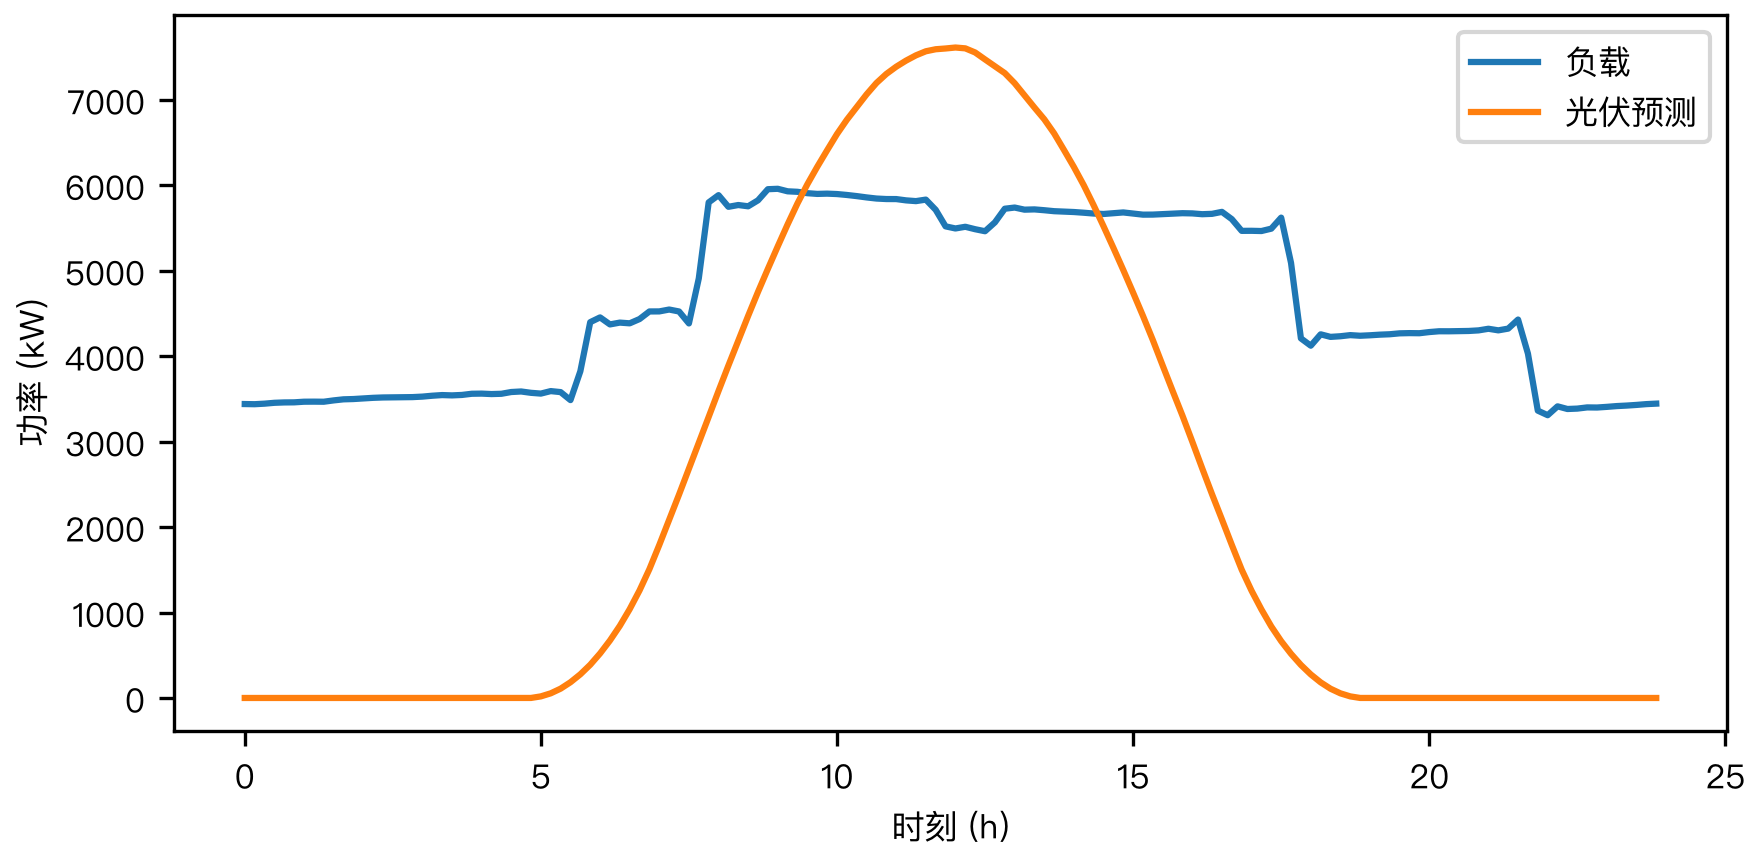
\includegraphics[width=.84\linewidth]{raw_q1_inputs.png}\caption{问题一输入序列}\label{fig:raw}\end{figure}

\section{统一物理模型}
令\(q_t,e_t,c_t,d_t,u_t\)分别为常规购电、紧急购电、交流侧充电、交流侧放电和未利用供能，单位为kWh；\(L_t,G_t\)为功率，\(p_t\)为交易价格。采用充电入库效率\(\eta=0.9\)和放电出库效率\(1/\eta\)，电池内部储能量为\(S_t\)。
\begin{equation}\label{eq:balance}
q_t+e_t+d_t+G_t\Delta t=L_t\Delta t+c_t+u_t .
\end{equation}
\begin{equation}\label{eq:soc}
S_{t+1}=S_t+\eta c_t-d_t/\eta .
\end{equation}
\begin{equation}\label{eq:bound}
0\le c_t,d_t\le 5000\Delta t,\quad 1200\le S_t\le10800,\quad S_0=6000 .
\end{equation}
问题一补充\(S_T=S_0\)和二元变量\(z_t\)，使\(c_t\le5000\Delta t z_t\)、\(d_t\le5000\Delta t(1-z_t)\)。Q2至Q4跨日传递前一日末状态。所有求解返回后检查非负性、功率上限、SOC边界和初始状态。微网调度的优化建模参考\cite{gulotta}，程序化优化表达参考\cite{pyomo}。

\section{问题一：确定性调度与库存价值}
问题一的目标为
\begin{equation}\label{eq:q1obj}
\min\sum_{t=0}^{143}p_tq_t,
\end{equation}
并令紧急购电为0。MILP得到全天购电量59482.699\,kWh、费用35126.986\,元，SOC范围为1200--10800\,kWh，日末回到6000\,kWh。图~\ref{fig:q1soc}展示互斥充放电与状态边界。
\begin{figure}[H]\centering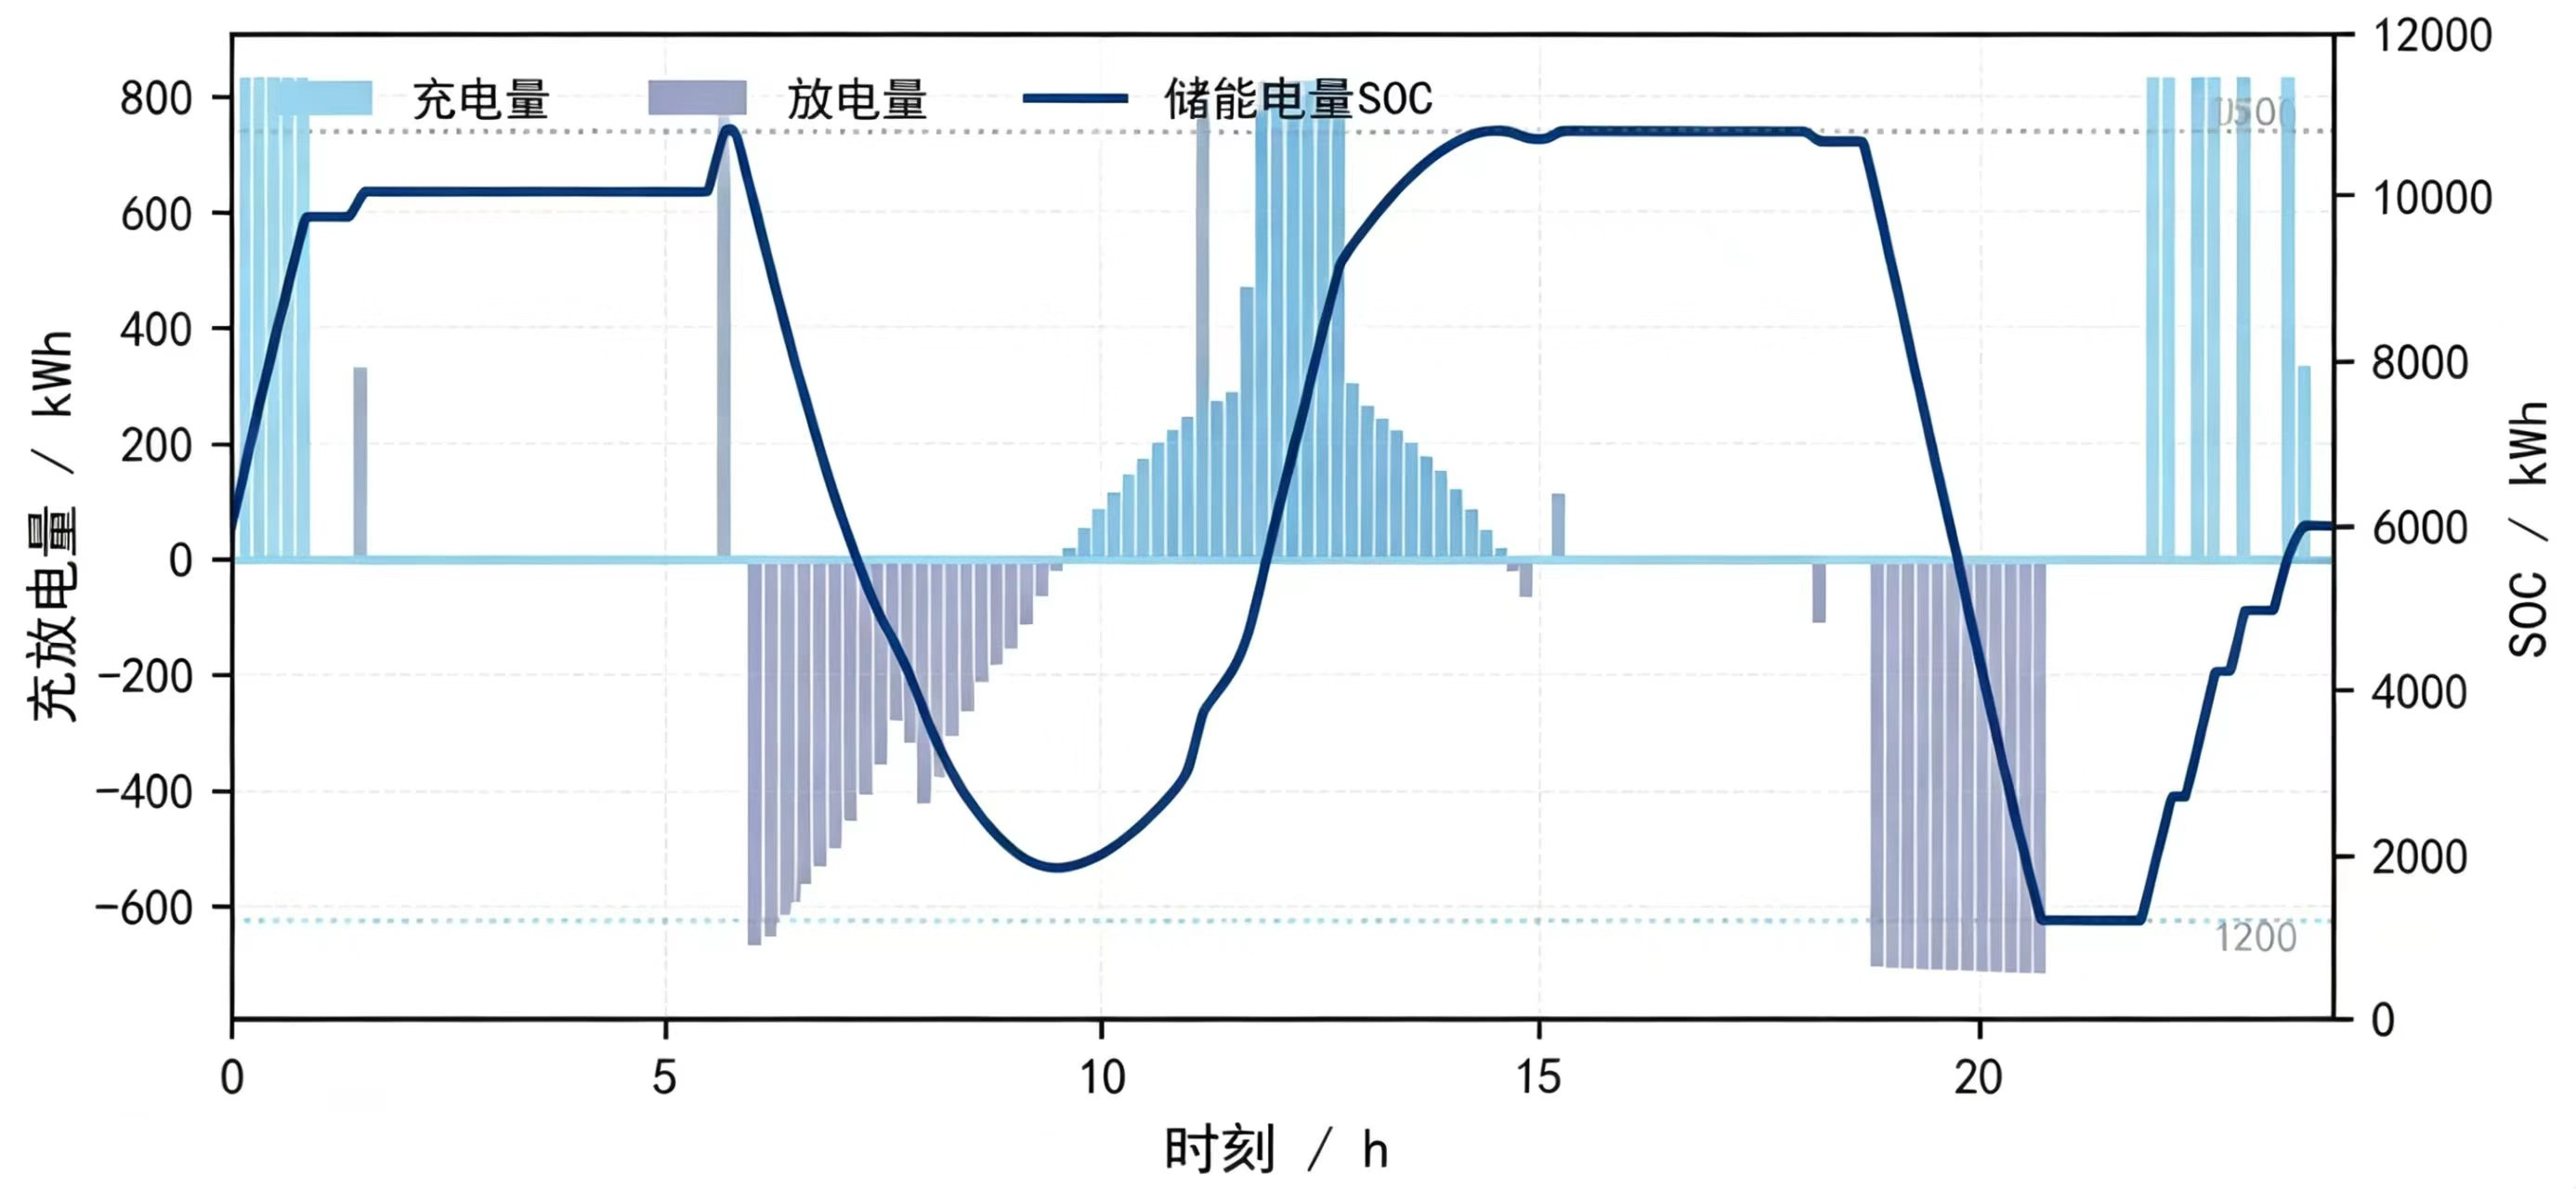
\includegraphics[width=.84\linewidth]{process_q1_soc.png}\caption{问题一充放电与SOC}\label{fig:q1soc}\end{figure}
为了检验单条最优轨迹之外的库存机会成本，另在5\,kWh网格上递推\(F_t(S)\)：
\begin{equation}\label{eq:dp}
F_t(S)=\min_{S\to S'}\{p_t\pos{N_t+c_t-d_t}+F_{t+1}(S')\},\qquad F_T(6000)=0 .
\end{equation}
其中\(N_t=(L_t-G_t)\Delta t\)。网格DP值为35188.908\,元，比MILP高0.1763\%，该差异是状态网格离散误差，故提交结果仍采用MILP。图~\ref{fig:q1dispatch}给出价格与购电量。
\begin{figure}[H]\centering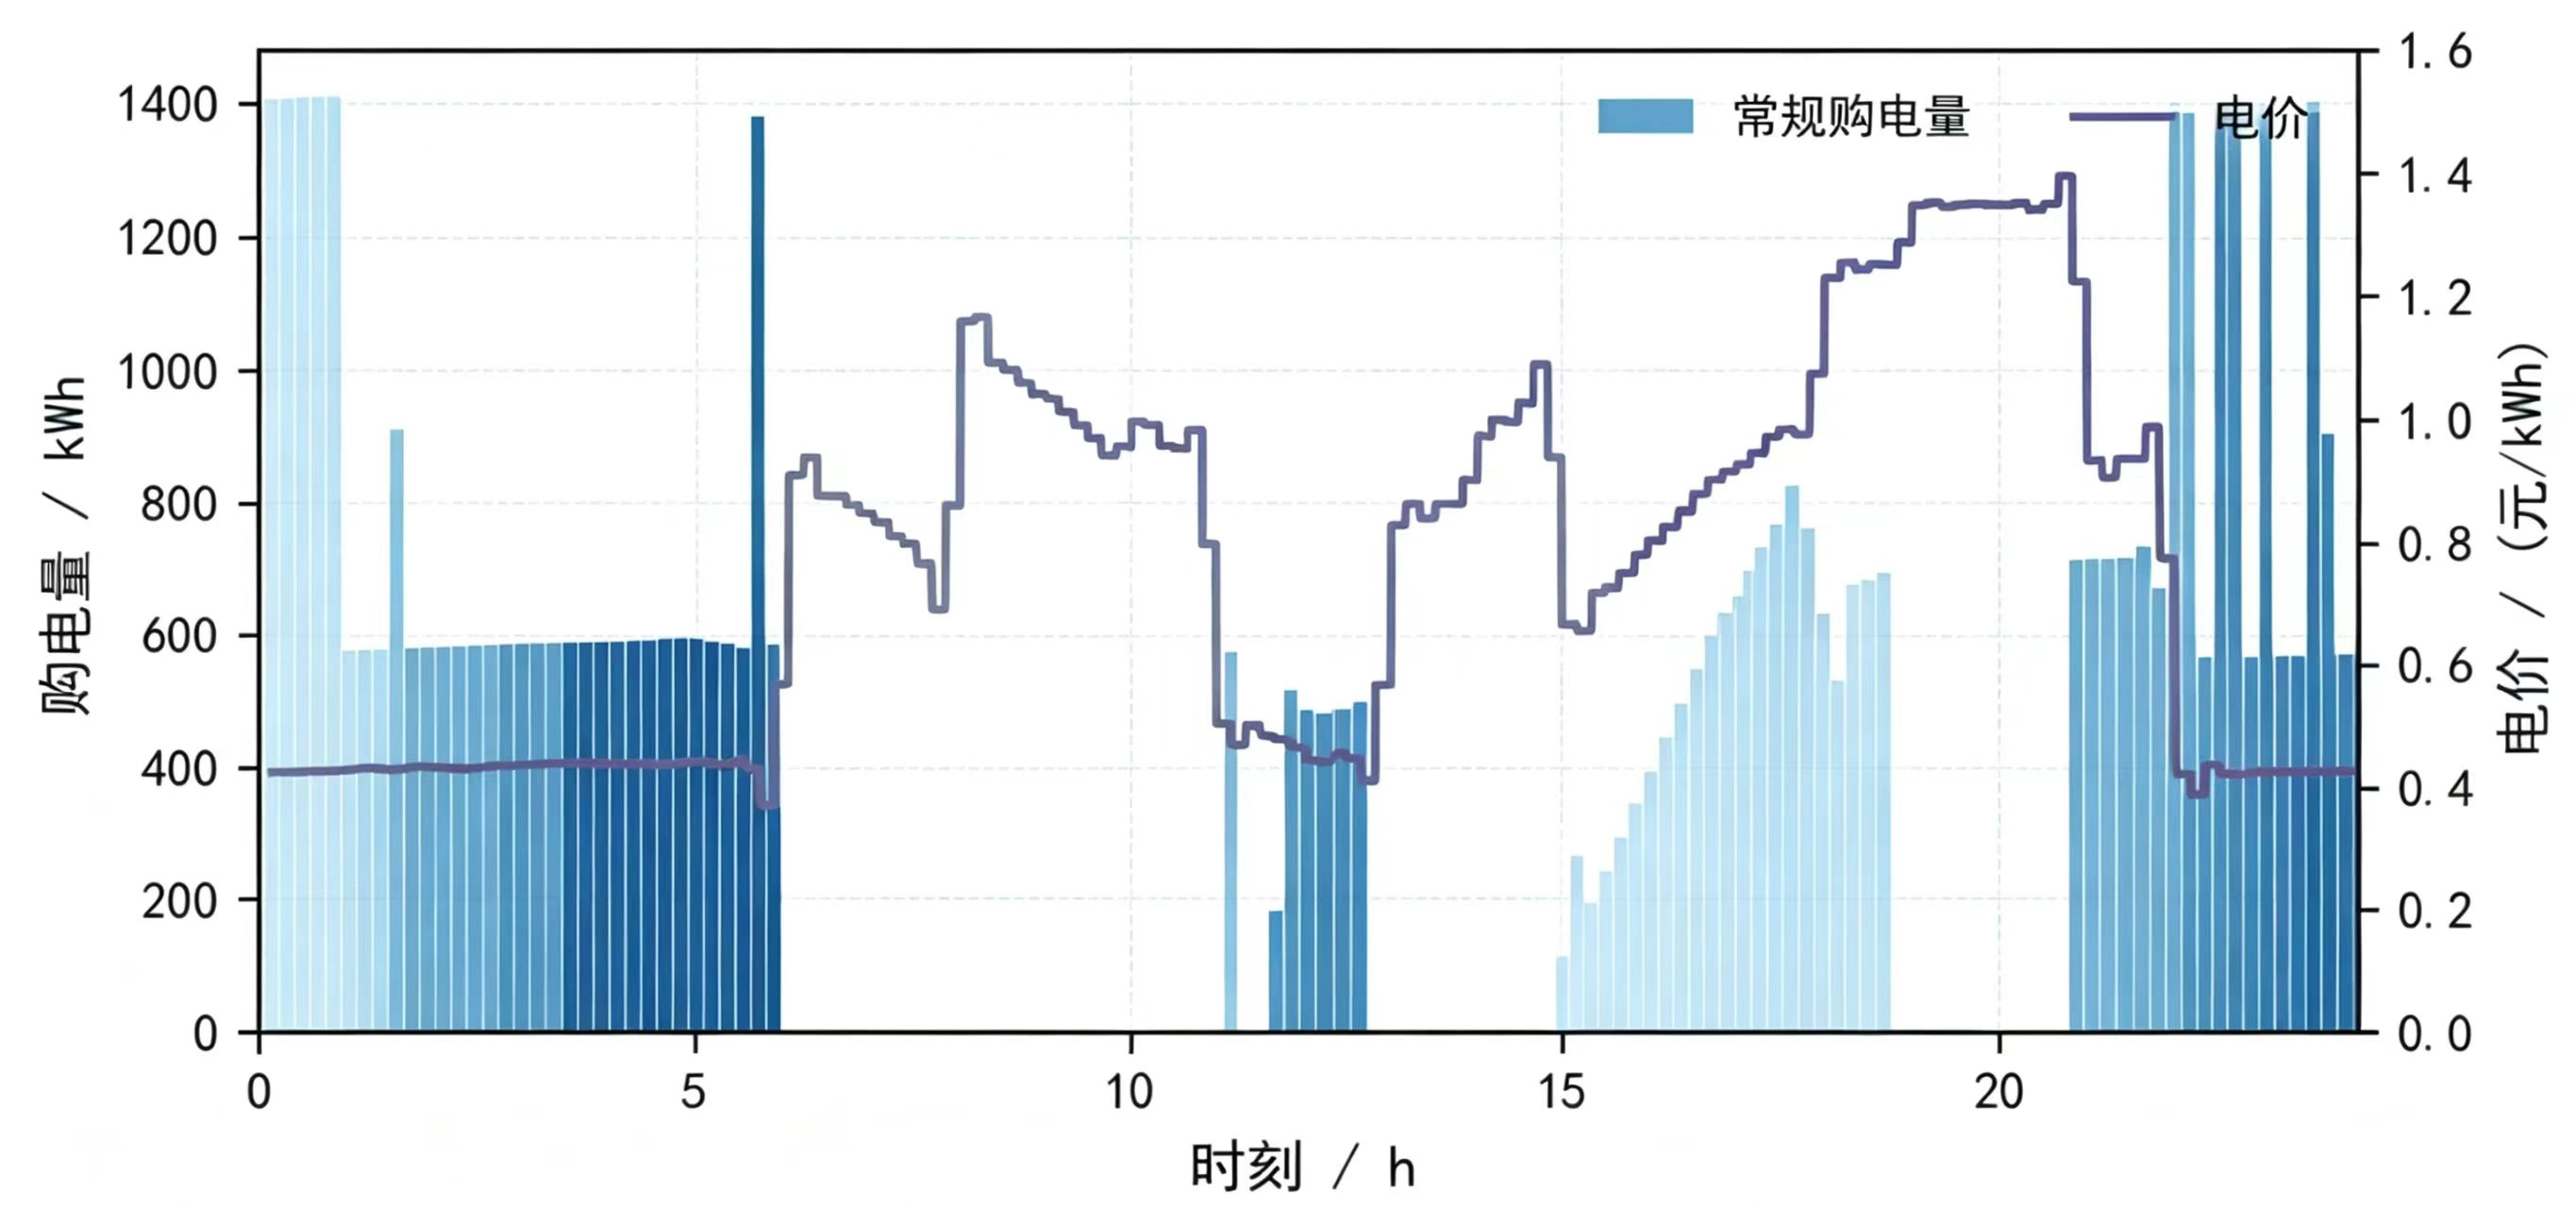
\includegraphics[width=.84\linewidth]{result_q1_dispatch.png}\caption{问题一价格与购电量}\label{fig:q1dispatch}\end{figure}

\section{问题二：日期因果回测}
负荷预测把历史同类型日的日电量水平与归一化日内形状分开估计：
\begin{equation}\label{eq:forecast}
\widehat L_{d,t}=\widehat B_d\widehat s_{d,t}/\Delta t,\qquad \sum_t\widehat s_{d,t}\Delta t=1 .
\end{equation}
光伏采用目标日前三日中位数并乘0.9。334天因果诊断显示，日电量—形状负荷MAPE为6.153\%，逐时七日中位数为17.987\%；三日和七日光伏中位数MAPE分别为4.027\%和4.697\%，详见\texttt{results/forecast\_diagnostics.csv}。计划使用预测量求解，实际缺口为
\begin{equation}\label{eq:emergency}
e_t=\pos{L_t\Delta t-G_t\Delta t-q_t-c_t+d_t} .
\end{equation}
Q2全年费用为16206550.45\,元，紧急购电量为789872.052\,kWh。图~\ref{fig:emergency}显示各场景的全年紧急购电量。
\begin{figure}[H]\centering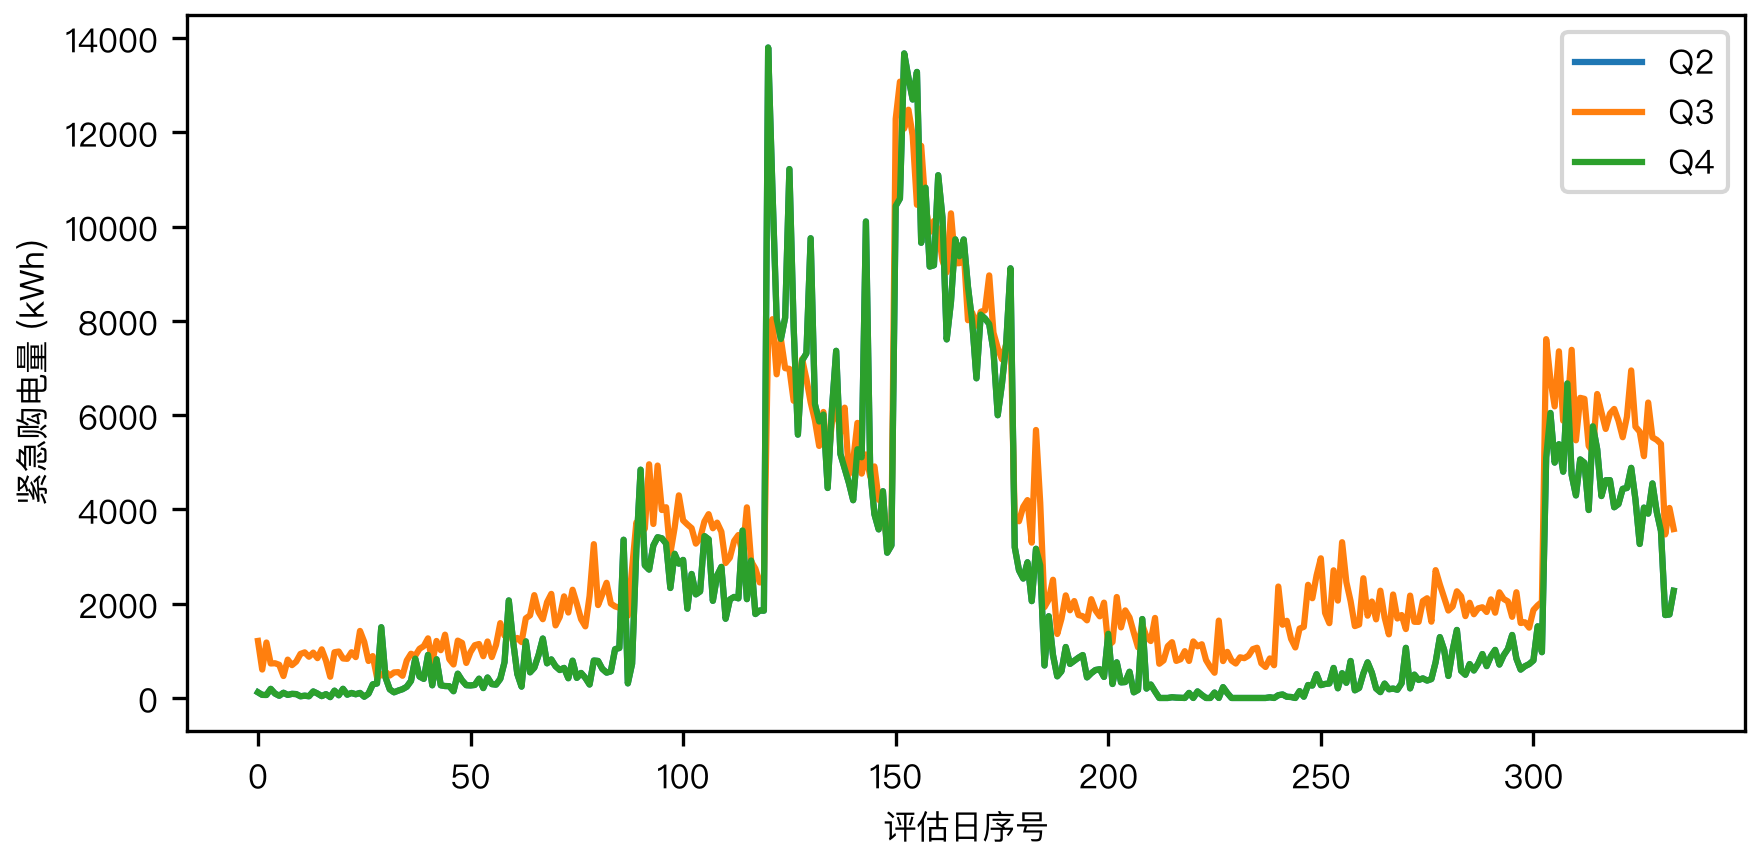
\includegraphics[width=.84\linewidth]{raw_q2_q3_q4_emergency.png}\caption{各场景全年紧急购电量}\label{fig:emergency}\end{figure}

\section{问题三：多时刻预报与B结算}
在0、6、12、18时只优化尚未执行的区间并锁定已执行前缀。设\(q_t^0\)为0时计划、\(q_t^a\)为调整计划，按题面文字采用
\begin{equation}\label{eq:settlement}
K_3=\sum_t p_tq_t^0+\sum_t0.5p_t\pos{q_t^0-q_t^a}+\sum_t1.5p_t\pos{q_t^a-q_t^0}+\sum_t5p_te_t .
\end{equation}
旧实现以\(q_t^a\)替代计划基准量会在调减时少算费用；本版本逐日写出基准费、调减费、调增费和紧急费，并用等式审计。Q3全年费用为18242015.85\,元，紧急购电量为1066446.282\,kWh。图~\ref{fig:adjust}展示调整幅度与紧急购电的关系。
\begin{figure}[H]\centering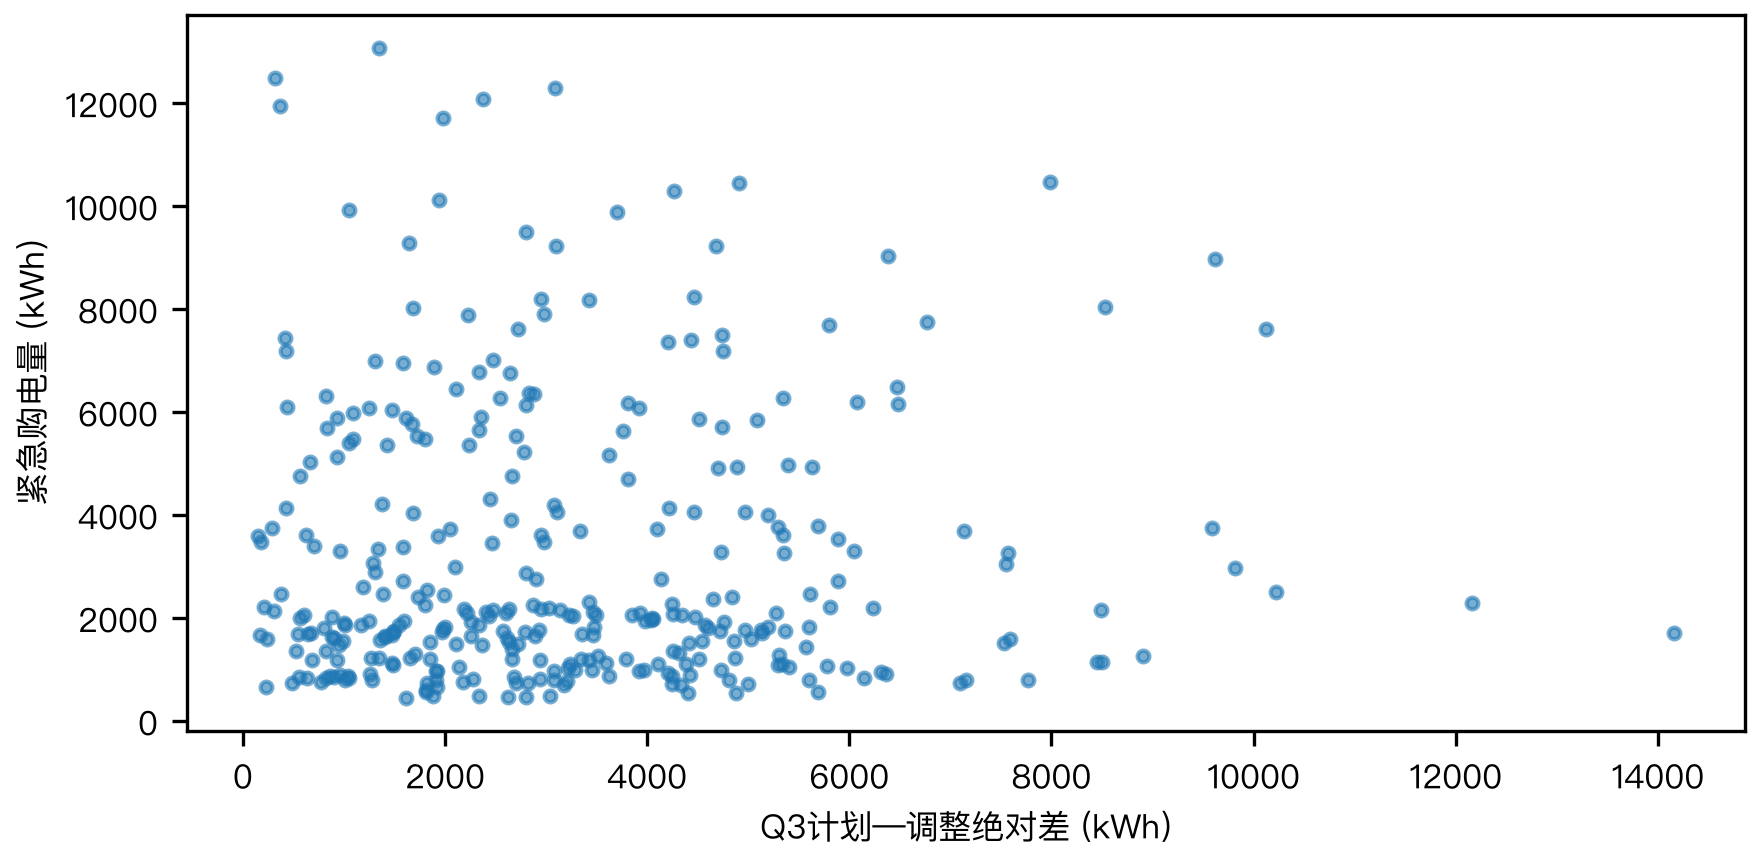
\includegraphics[width=.84\linewidth]{process_q3_adjustment.png}\caption{问题三计划—调整差额}\label{fig:adjust}\end{figure}

\section{问题四：波动价格与独立分支}
Q4-2将附件4价格替换固定价格并沿用Q2的信息边界；Q4-3沿用Q3的四次滚动预报和式~\eqref{eq:settlement}。两分支从每天相同的日初SOC独立启动，避免把Q4-2的日末状态带入Q4-3。结果汇总于表~\ref{tab:annual}，日费用分布与Q4-3序列见图~\ref{fig:box}和图~\ref{fig:q43}。
\begin{table}[H]\centering\caption{全年本地回测结果}\label{tab:annual}
\begin{tabular}{lrr}\toprule 场景&费用/元&紧急购电/kWh\\\midrule
Q2&16206550.45&789872.052\\
Q3&18242015.85&1066446.282\\
Q4-2&16989713.48&789872.052\\
Q4-3&19577410.54&1067444.696\\\bottomrule\end{tabular}\end{table}
\begin{figure}[H]\centering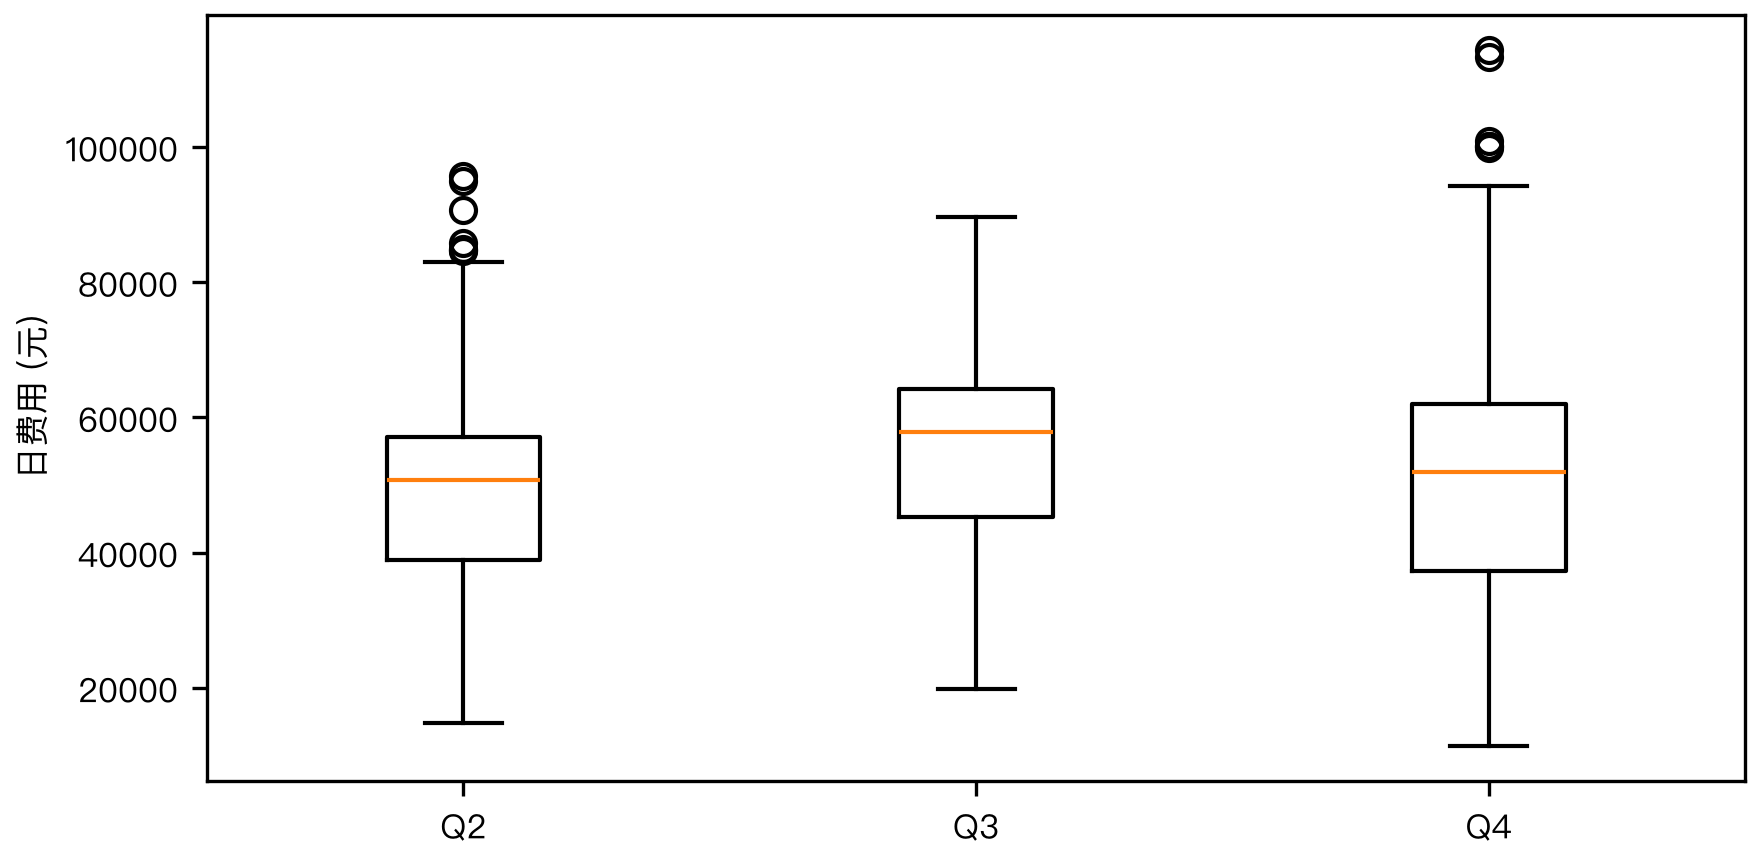
\includegraphics[width=.84\linewidth]{result_q4_cost_box.png}\caption{各场景日费用分布}\label{fig:box}\end{figure}
\begin{figure}[H]\centering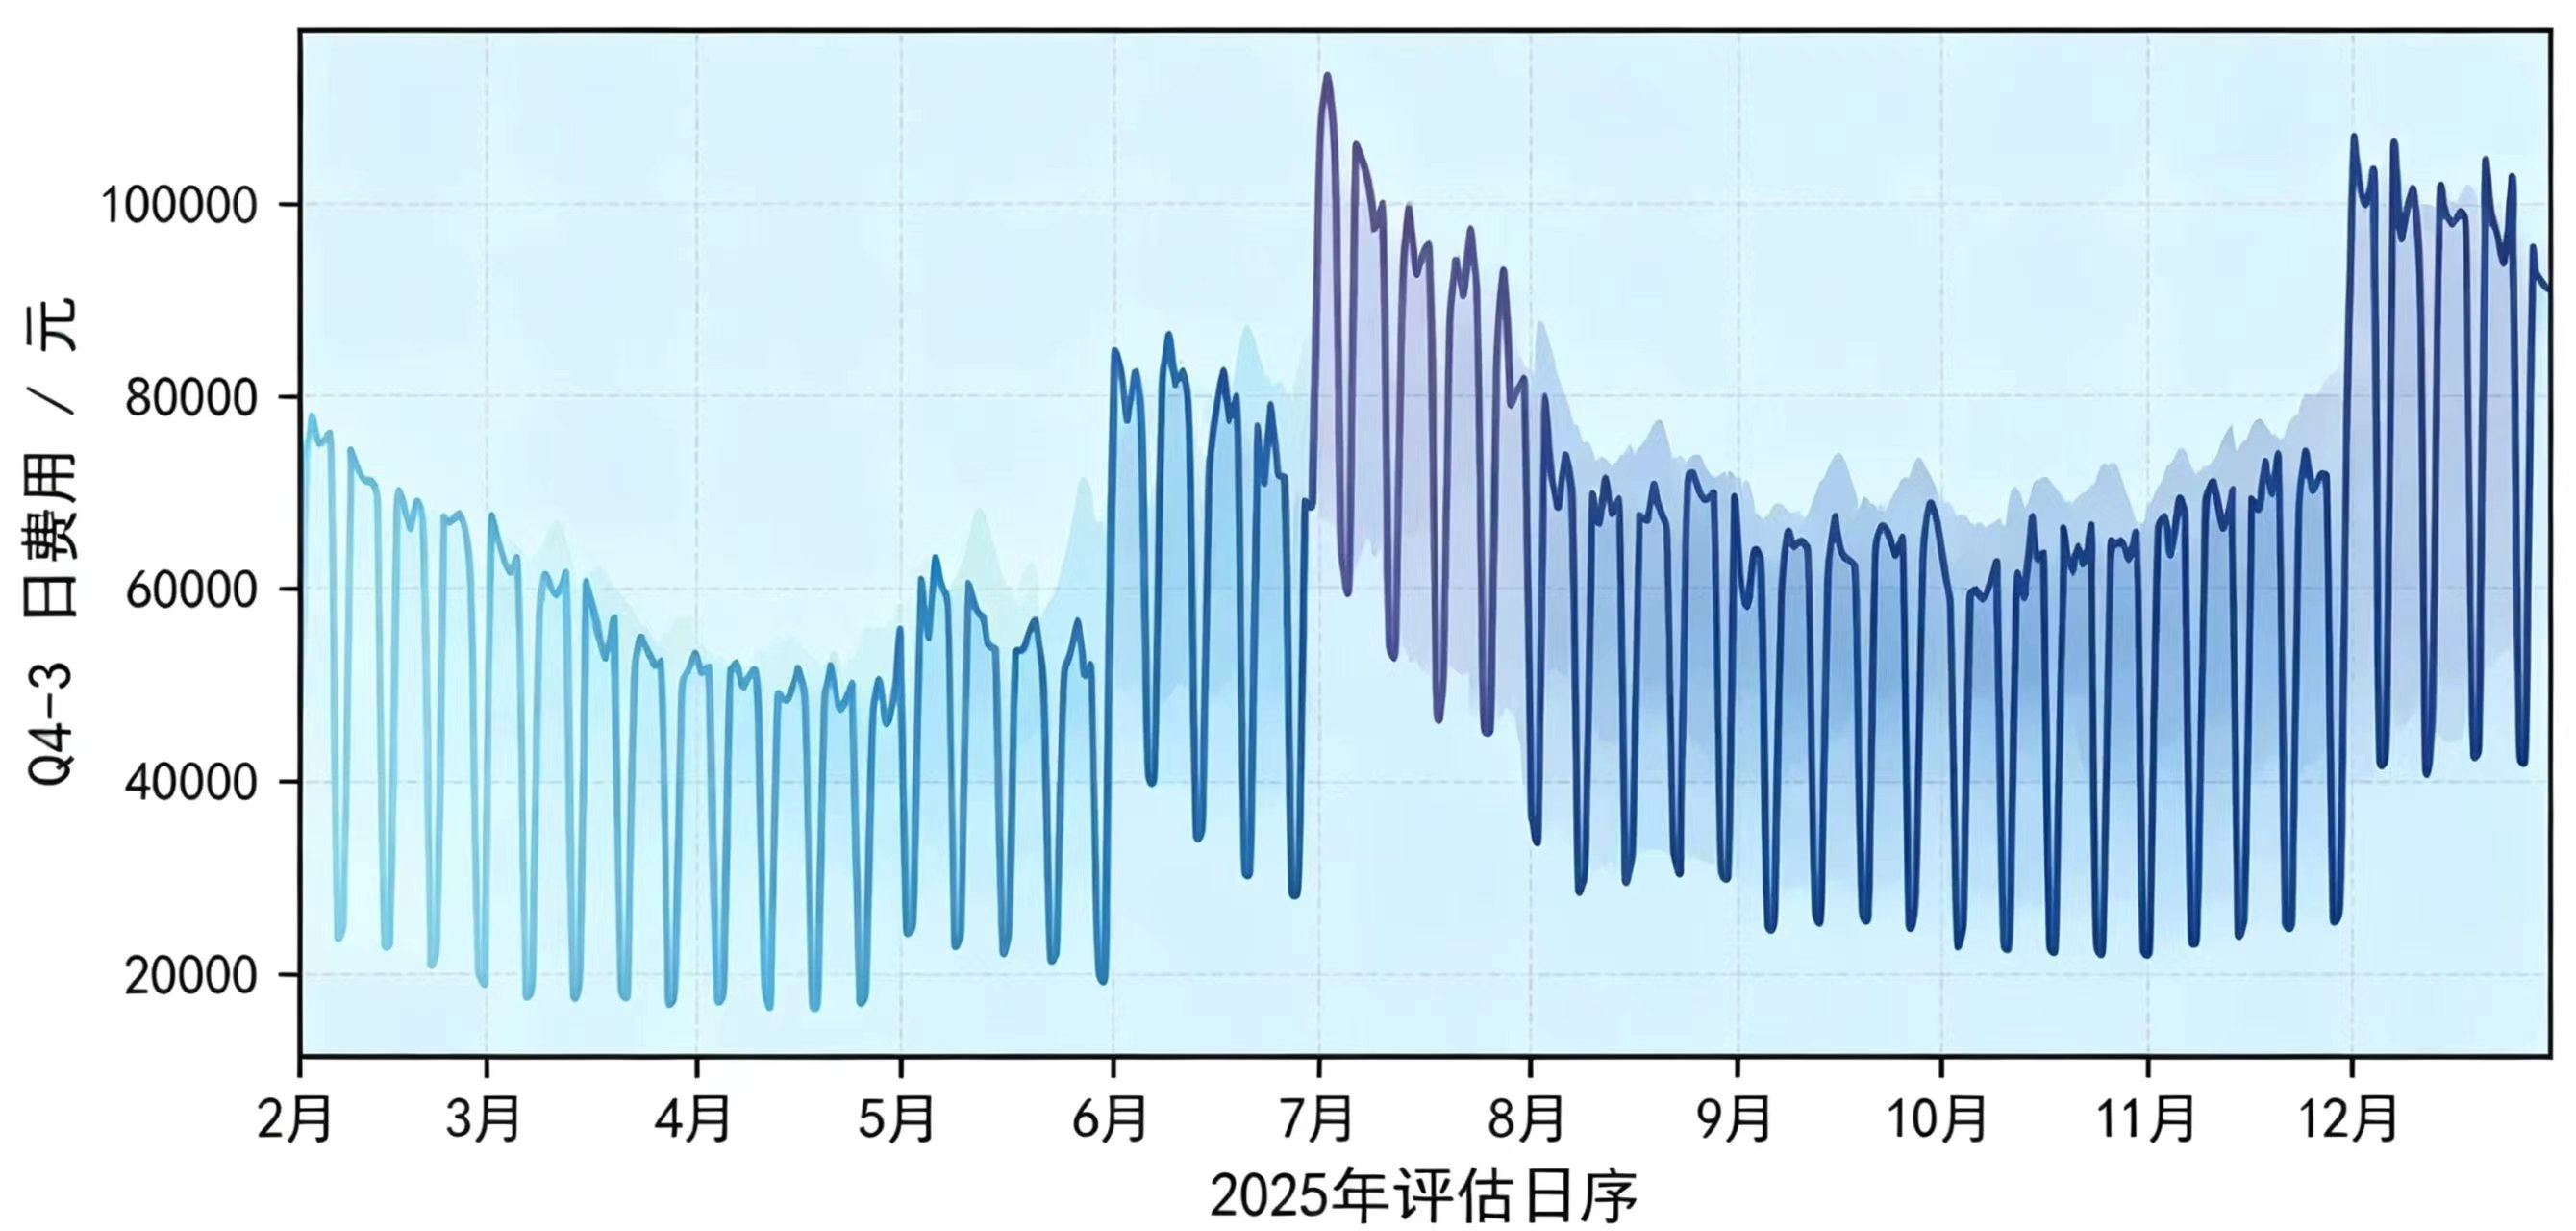
\includegraphics[width=.84\linewidth]{result_q4_3_series.png}\caption{问题4-3逐日费用}\label{fig:q43}\end{figure}

\section{敏感性、对抗性检查与局限}
光伏保守系数敏感性见表~\ref{tab:sens}。在日电量—形状负荷预测下，0.9系数的全年费用低于0.8和1.0；这只是当前附件回测结果，不是普适最优系数。
\begin{table}[H]\centering\caption{Q2光伏保守系数敏感性}\label{tab:sens}
\begin{tabular}{lrr}\toprule 系数&费用/元&紧急购电/kWh\\\midrule
0.80&16622826.83&627200.633\\
0.90&16206550.45&789872.052\\
1.00&17440007.68&1333753.169\\\bottomrule\end{tabular}\end{table}
本版本对外部经验材料采取以下边界：经验材料的数字不直接引用；知道未来情景的递推只能作为规划近似，不能证明因果执行；LP互斥结论只在非负价格、允许弃用富余供能等假设下成立；Q3结算按题面逐项核算；Q4-2和Q4-3保持独立分支。当前版本尚未引入完整非预见性场景树、通信延迟、电池退化和CVaR风险度量，故所有全年数字均标为本地附件回测。

\section{结论与可复现性}
统一模型覆盖四个问题，MILP提供可执行购电轨迹，网格DP提供库存价值的独立数值检查，日电量—形状预测减少负荷预测偏差，滚动调整反映预报信息进入后的再决策，独立价格分支避免状态污染。唯一复现命令为：
\begin{verbatim}
../.venv/bin/python solve_c.py --seed 20260911
\end{verbatim}
结果表位于\texttt{results/result*.xlsx}，逐日账单位于\texttt{results/daily\_metrics.csv}，预测诊断位于\texttt{results/forecast\_diagnostics.csv}，输入哈希和环境记录位于\texttt{results/复现清单.json}。

\section*{AI工具使用声明}
Codex用于资料检索、代码组织、公式排版和结果复核；参赛队员负责题面解释、模型假设、参数选择、代码运行、结果解释和最终提交。外部经验贴和附件论文仅作为思路参考，未被当作官方规则或未经复现的结果来源。

\begin{thebibliography}{9}
\bibitem{cumcm} 全国大学生数学建模竞赛组委会. 2026年竞赛题目及人工智能使用规定（以官方发布版本为准）.
\bibitem{gulotta} Gulotta T, et al. Microgrid energy management under uncertainty. International Journal of Electrical Power \& Energy Systems, 2023.
\bibitem{pyomo} Hart W E, et al. Pyomo—optimization modeling in Python. Springer, 2017.
\end{thebibliography}
\end{document}
